\documentclass[tikz,border=5mm]{standalone}
\usetikzlibrary{shapes.geometric, arrows, positioning, fit, calc}

\begin{document}
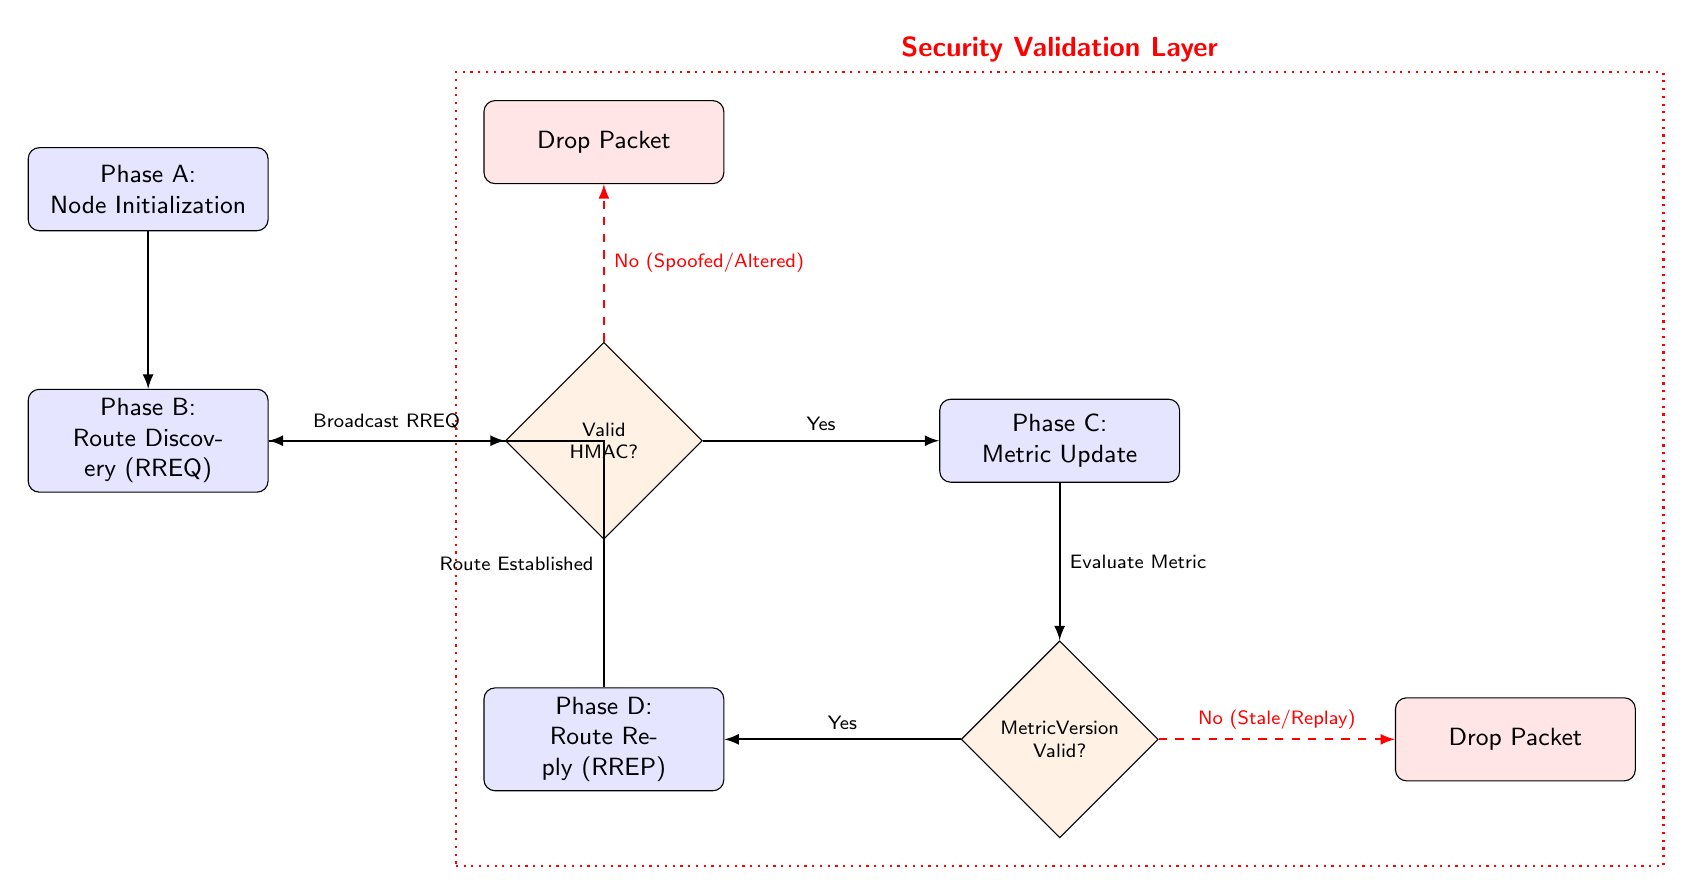
\begin{tikzpicture}[
		node distance=2cm and 3cm,
		block/.style={rectangle, draw, fill=blue!10, text width=8em, text centered, rounded corners, minimum height=3em, font=\sffamily\small},
		validation/.style={diamond, draw, fill=orange!10, text width=4.5em, text centered, minimum height=4em, font=\sffamily\scriptsize},
		line/.style={draw, -latex, thick},
		dashed_line/.style={draw, -latex, dashed, thick},
		highlight/.style={draw, red, thick, text=red}
	]

	% Phase A: Initialization
	\node [block] (init) {Phase A:\\Node Initialization};

	% Phase B: Route Discovery
	\node [block, below=of init] (rreq) {Phase B:\\Route Discovery (RREQ)};

	% Validation Gate 1
	\node [validation, right=of rreq] (val1) {Valid\\HMAC?};

	% Phase C: Metric Update
	\node [block, right=of val1] (metric) {Phase C:\\Metric Update};

	% Validation Gate 2
	\node [validation, below=of metric] (val2) {MetricVersion\\Valid?};

	% Phase D: Route Reply
	\node [block, left=of val2] (rrep) {Phase D:\\Route Reply (RREP)};

	% Drop states
	\node [block, fill=red!10, above=of val1] (drop1) {Drop Packet};
	\node [block, fill=red!10, right=of val2] (drop2) {Drop Packet};

	% Edges
	\path [line] (init) -- (rreq);
	\path [line] (rreq) -- node[above, font=\sffamily\scriptsize] {Broadcast RREQ} (val1);
	\path [line] (val1) -- node[above, font=\sffamily\scriptsize] {Yes} (metric);
	\path [dashed_line, red] (val1) -- node[right, font=\sffamily\scriptsize] {No (Spoofed/Altered)} (drop1);

	\path [line] (metric) -- node[right, font=\sffamily\scriptsize] {Evaluate Metric} (val2);
	\path [line] (val2) -- node[above, font=\sffamily\scriptsize] {Yes} (rrep);
	\path [dashed_line, red] (val2) -- node[above, font=\sffamily\scriptsize] {No (Stale/Replay)} (drop2);

	\path [line] (rrep) |- node[near start, left, font=\sffamily\scriptsize] {Route Established} (rreq);

	% Highlighting the validation points
	\node[draw=red, thick, dotted, fit=(val1)(val2)(drop1)(drop2), inner sep=1em] (box) {};
	\node[above, text=red, font=\sffamily\bfseries] at (box.north) {Security Validation Layer};

\end{tikzpicture}
\end{document}